\section{Задача прогнозирования временных рядов}
\label{sec:purpose}

Прогнозирование временных рядов является одним из важных факторов предсказания будущих значений, анализе трендов, циклов и сезонностей в определённых
значениях. Для начала, следует рассмотреть само понятие временного ряда.

Временной ряд: \begin{equation}\label{timeline_value} Y_1, Y_2 ... Y_t \in \mathbf{R}  \end{equation}, значения признака, измеренные через постоянные временные интервалы \cite{wiki}.

Ключевая особенность состоит в том, что измерения признака происходит во времени и между разными измерениями всегда проходит одинаковое количество времени.
Т.к. если промежуток между отсчётами будет случайным, то в этом случае это будет являться случайным процессом и методы для обработки будут использоваться другие, нежели
при работе с прогнозированием временных рядов.

В данном случае, мы рассматриваем прогнозирование вещественного скалярного ряда, т.е. измерения принадлежат множеству вещественных чисел ($R$).

Как простой пример временного ряда можно рассмотреть временной ряд заработных плат \cite{datamining_in_action}.

\begin{figure}[h]
\centering
	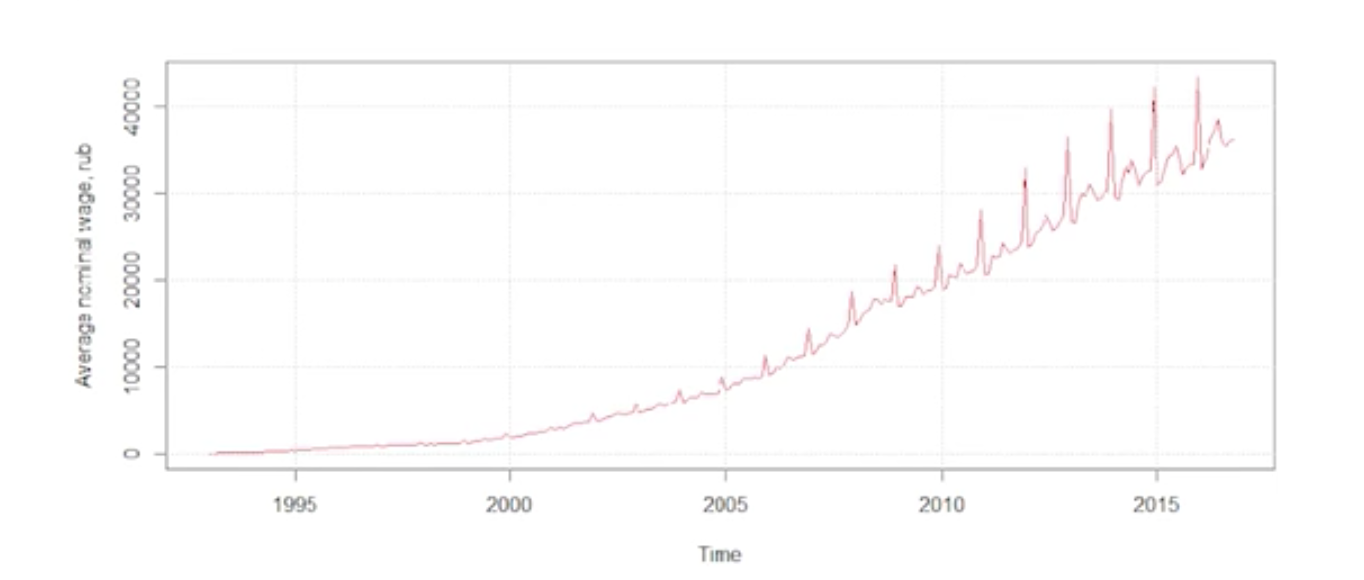
\includegraphics[totalheight=7cm]{main_part/timeline-payings.png}
	\caption{Пример временного ряда}
	\label{sec:purpose:payings}
\end{figure}

На данном рисунке видно, что, есть тренд к росту зарплат и пики, в декабре - месяце, где выдаются годовые премии. Длина ряда не является фиксированной величиной и может меняться, день, неделя, месяц, квартал, год. Сам по себе промежуток не имеет значения при прогнозировании.

Задачей прогнозирования временных рядов является поиск функции F, которая будет будет зависеть от всей известной информации к моменту прогнозирования, который обозначается $ T $. На вход данная функция принимает все значения ряда, от $ Y_1$ до $ Y_t $. Также, функция принимает дополнительный параметр $ H $, который показывает насколько вперёд необходимо прогнозировать ряд. Параметр $h$ принимает значения от 1 до $ H $ ($ h \in {1, 2, ... H} $), где $ H $ называется горизонтом прогнозирования.

Помимо прогнозов, которые представляют собой число, при прогнозировании полезно добавлять интервал, который показывает вероятность, с которой будет выполнено предсказание.
Такой интервал называется предсказательным. 

Предсказательный интервал - интервал, в котором предсказываемая величина окажется с вероятностью не меньше заданной. В данном случае, не стоит его путать с доверительным интервалом, который является случайным интервалом, для фиксированного неслучайного параметра. Предсказательный интервал является очень полезным инструментом, т.к. он показывает заказчику прогноза, насколько можно быть уверенным в произведённом прогнозе. И в данном случае важно, данную степень неуверенности квантифицировать.

Как пример: в апреле 1997 в городе Гранд-Фокс, Северная Дакота, произошло наводнение. Город был защищён дамбой высотой 51 фут, согласно прогнозу, высота паводка должна была составить 49 футов, истинная же высота, оказалась 54. В результате этой ошибки было эвакуировано 75\% населения города и нанесён ущерб на несколько миллиардов долларов. На исторических данных, точность прогнозов метеорологической службы составляла +- 9 футов.

Таким образом, выделим особенности задачи прогнозирования временных рядов:
\begin{itemize}
	\item в классических задачах анализа данных предполагается независимость наблюдений;
	\item при прогнозировании временных рядов, прогноз строится на исторических данных.
\end{itemize}

В отличии от задач машинного обучения и статистики, где значения, как правило, являются простой выборкой, т.е. разные наблюдения, померенные на разных объектах, независимые одинаково распределённые. В то время как при прогнозировании временных рядов, данные устроены принципиально по другому - будущее зависит от прошлого, т.е. чем меньше прошлое похоже на шум, тем точнее можно будет сделать прогноз.

Лучше всего, в машинном обучении, решаются задачи с учителем, т.е. есть определённом количество признаков и выходы, для данных признаков. В данном же случае, прогнозирования временных рядов, отсутсвуют $ x $-ы, т.е. отсутствуют признаки, есть только $y$-ки \cite{datamining_in_action}.

\begin{figure}[h]
\centering
	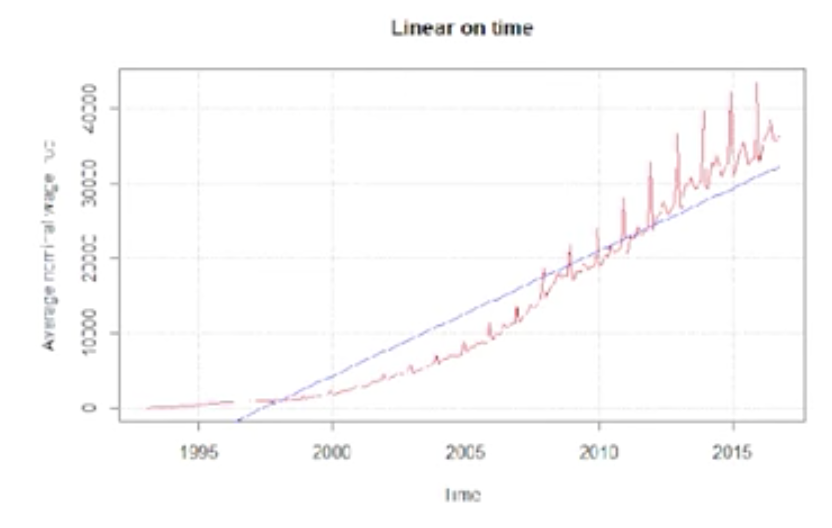
\includegraphics[totalheight=7cm]{main_part/linear-on-time.png}
	\caption{Применение методов машинного обучения (линейное)}
	\label{sec:purpose:linear}
\end{figure}

В данном рисунке видно, что предсказания (синяя линия) не будут достаточно точными, т.к. они явно не учитывают нешумовые всплески \cite{datamining_in_action}.

\begin{figure}[h]
\centering
	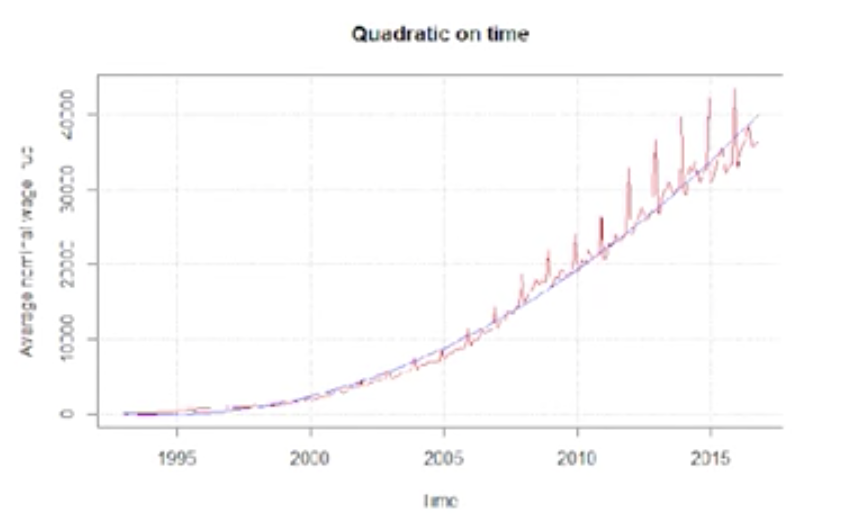
\includegraphics[totalheight=7cm]{main_part/quadratic-on-time.png}
	\caption{Применение методов машинного обучения (квадратичное)}
	\label{sec:purpose:quadratic}
\end{figure}

Также и применение квадратичной функции не приводит к точному предсказанию.

Ключевая особенность временного ряда заключается в том, что соседние значения не независимы. Квантифицировать это можно с помощью автокорреляции. Автокорреляция, это корреляция ряда с самим собой, сдвинутым на определённое количество отсчётов. То количество, на которое мы сдвигаем отсчёт, называется \textit{лагом} автокорреляции. Автокорреляция меняет свои значения от -1 до 1, 1 означает идеальную линейную зависимость с положительным знаком, -1 - линейная зависимость с отрицательным, 0 - отсутствие линейной зависимости.

Также необходимо рассмотреть компоненты временных рядов, т.е. то, из чего состоят ряды.

\textit{Тренд} - плавное долгосрочное среднего изменения уровня ряда. Ряд может <<колебаться>> вокруг своего тренда.

\textit{Сезонность} - циклические изменения уровня ряда с постоянным периодом. Например, если рассматриваются месячные ряды, то в них, скорее всего, будет годовая сезонность, т.е. то, что происходит в декабре этого года, будет похоже на то, что происходило в декабре предыдущего года.

\textit{Цикл} - изменения уровня ряда с переменным периодом (например экономические циклы, периоды солнечной активности).

\textit{Ошибка} - непрогнозируемая случайная компонента ряда.

Ошибку, также, можно описать как то, что нельзя описать любыми другими компонентами ряда. Рассмотрим несколько примеров.

В данном ряде можно рассмотреть тренд к падению количества контрактов сокровищницы США по дням \cite{datamining_in_action}.

\begin{figure}[h]
\centering
	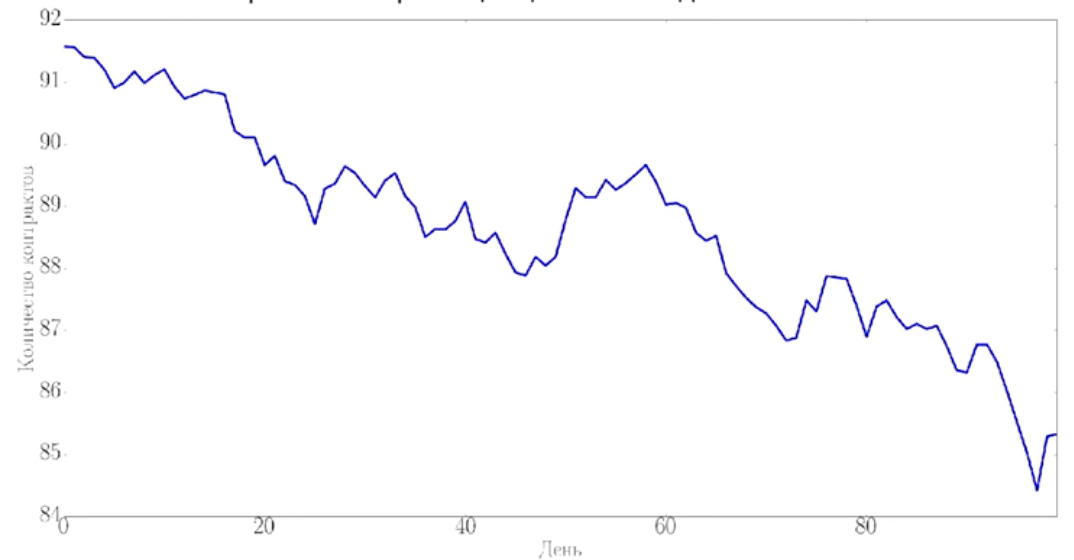
\includegraphics[totalheight=7cm]{main_part/usa-gold.png}
	\caption{Количества контрактов сокровищницы США}
	\label{sec:purpose:contracts}
\end{figure}

Это ряд, в котором можно отметить линейно понижающийся тренд. Можно сказать, что ряд совершает <<колебания>> вокруг своей линии тренда.

Далее можно рассмотреть ряд с объёмами производства электричества в Австралии \cite{datamining_in_action}.

\begin{figure}[h]
\centering
	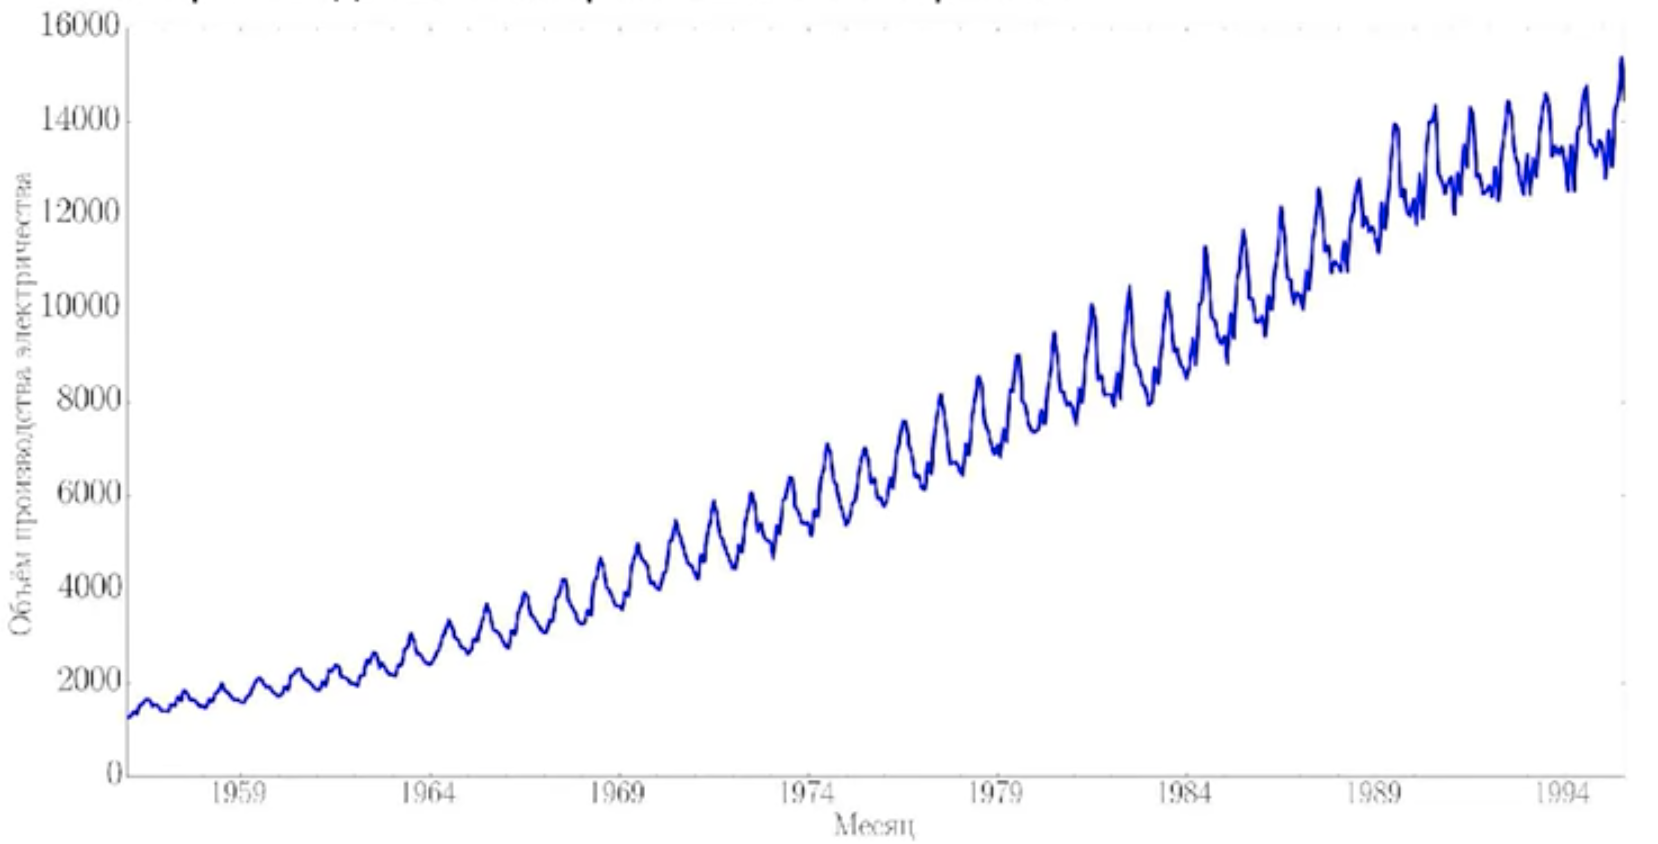
\includegraphics[totalheight=7cm]{main_part/australia-electricity.png}
	\caption{Объём производства электричества в Австралии}
	\label{sec:purpose:electricity}
\end{figure}

В данном ряде есть ярковыраженный повышающийся тренд и кроме того, сильная годовая сезонность. Хорошо видно, что на графике происходят колебания на середину лета - зиму в Австралии, с повышением потребления электричества.

На следующем графике представлен временной ряд продажи жилых домов \cite{datamining_in_action}.

\begin{figure}[h]
\centering
	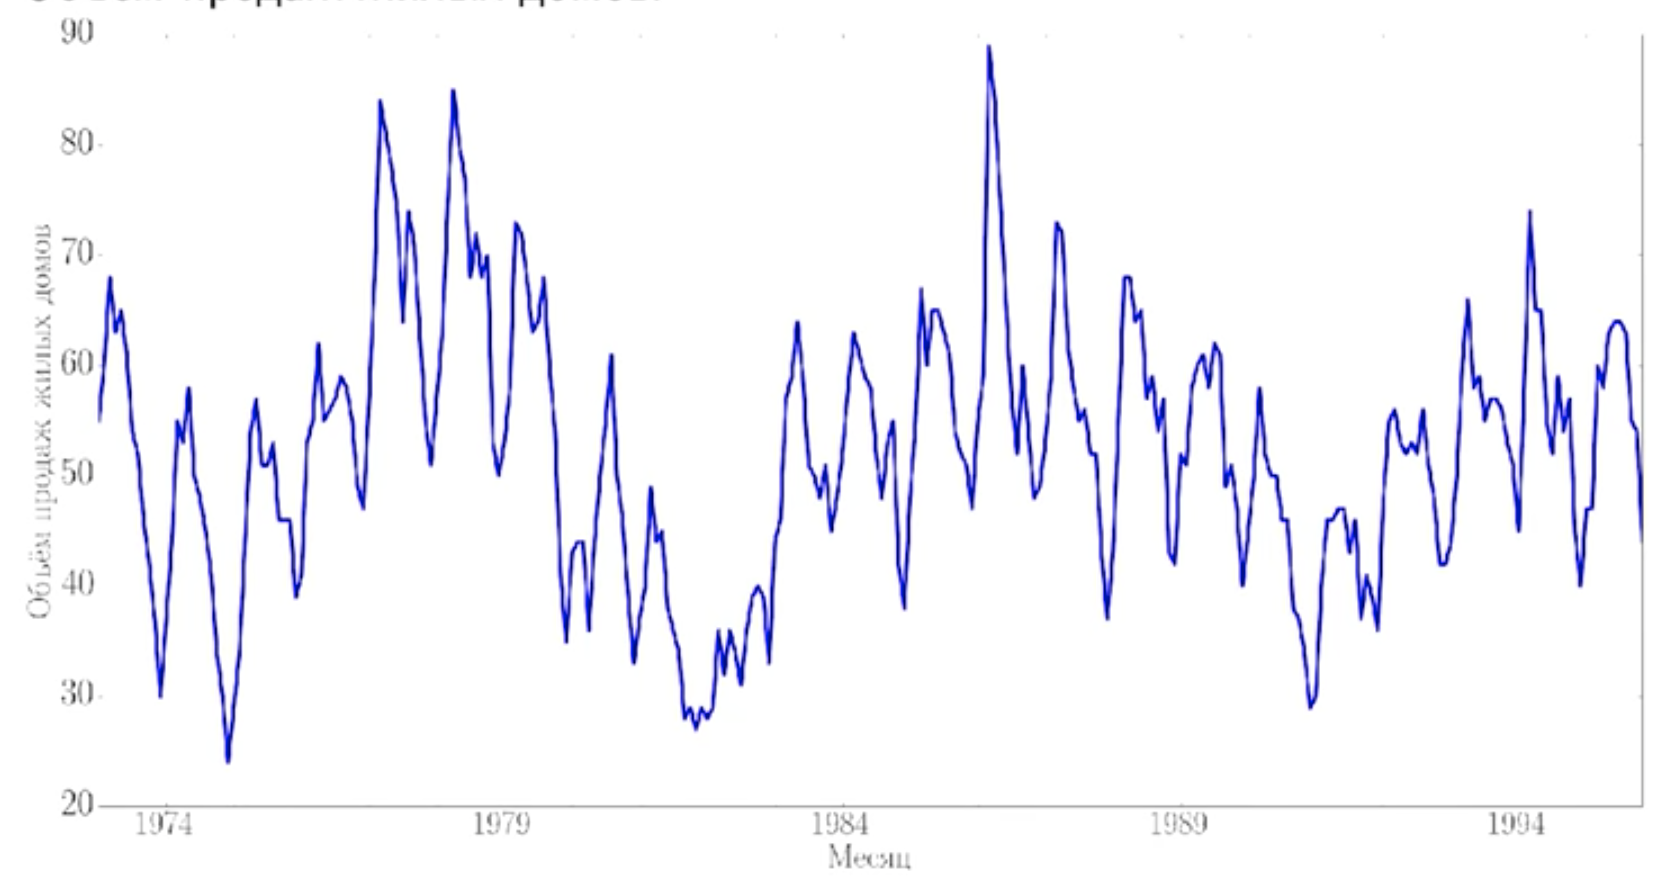
\includegraphics[totalheight=7cm]{main_part/house-sells.png}
	\caption{Объём продажи жилых домов в США}
	\label{sec:purpose:house-sells}
\end{figure}

На данном графике можно заметить годовую сезонность, длиной премерно равной году, и экономические циклы, которые можно отметить спадами и подъёмами объёмов продаж с нефиксированной временной длиной.




